% fig1-mcts-tree.tex
% MCTS Proof Search Tree (Cleaned)
\documentclass[tikz,border=9pt]{standalone}

% common-styles.tex
% Shared TikZ styles for wonton-proof paper figures

\usepackage{silence}
\WarningFilter{latex}{Missing character} 
\tracinglostchars=0 % Suppress engine-level "Missing character" warnings

\usepackage{fontspec}
\usepackage{unicode-math}

% Use filenames for reliability with Tectonic
\setmainfont{LibertinusSerif-Regular.otf}[
    BoldFont=LibertinusSerif-Bold.otf,
    ItalicFont=LibertinusSerif-Italic.otf,
    BoldItalicFont=LibertinusSerif-BoldItalic.otf
]
\setsansfont{LibertinusSans-Regular.otf}[
    BoldFont=LibertinusSans-Bold.otf,
    ItalicFont=LibertinusSans-Italic.otf
]
\setmonofont{LibertinusMono-Regular.otf}

% Try a more standard math font if LibertinusMath is causing nullfont issues
\setmathfont{LibertinusMath-Regular.otf}
% \setmathfont{latinmodern-math.otf}[range=digits] 

\usepackage{amsmath}
\usepackage{tikz}
\usepackage{forest}

\usetikzlibrary{
    arrows.meta,
    calc,
    decorations.pathreplacing,
    fit,
    positioning,
    shapes.geometric,
    shapes.misc,
    backgrounds,
    shadows.blur,
    fadings
}

% Color palette (muted, print-friendly)
\definecolor{ink}{RGB}{45,45,52}
\definecolor{muted}{RGB}{115,115,125}
\definecolor{highlight}{RGB}{198,120,44}
\definecolor{accentblue}{RGB}{86,130,178}
\definecolor{accentgreen}{RGB}{84,156,132}
\definecolor{blocked}{RGB}{140,75,75}
\definecolor{goalnode}{RGB}{255,255,255}
\definecolor{terminal}{RGB}{238,239,244}
\definecolor{deadnode}{RGB}{248,245,245}
\definecolor{flowbox}{RGB}{250,250,252}
\definecolor{basin1}{RGB}{224,234,248}
\definecolor{basin2}{RGB}{246,232,221}
\definecolor{basin3}{RGB}{228,242,234}
\definecolor{heatbase}{RGB}{86,130,178}

\tikzset{
    line cap=round,
    line join=round,
    pop/.style={
        blur shadow={shadow blur steps=5, shadow blur extra rounding=1.3pt}
    },
    base node/.style={
        rounded rectangle,
        draw=ink,
        line width=0.6pt,
        fill=goalnode,
        text=ink,
        minimum width=2.2cm,
        minimum height=0.7cm,
        align=center,
        pop
    },
    goal/.style={base node, fill=goalnode},
    terminal/.style={base node, fill=terminal, line width=0.9pt},
    dead/.style={base node, fill=deadnode, dashed},
    flowbox/.style={
        rectangle,
        draw=muted,
        rounded corners=3pt,
        fill=flowbox,
        minimum width=1.8cm,
        minimum height=0.6cm,
        align=center,
        font=\normalfont\small,
        text=ink,
        pop
    },
    decision/.style={
        diamond,
        draw=muted,
        fill=flowbox,
        aspect=2.4,
        font=\normalfont\small,
        inner sep=1pt,
        text=ink
    },
    protocolbox/.style={
        rectangle,
        draw=muted,
        rounded corners=4pt,
        fill=flowbox,
        minimum width=2cm,
        minimum height=0.8cm,
        font=\normalfont\small,
        align=center,
        text=ink
    },
    tactic/.style={
        ->,
        >=Stealth,
        draw=muted,
        line width=0.75pt
    },
    tacticlight/.style={
        ->,
        >=Stealth,
        draw=muted!45,
        dashed,
        line width=0.6pt
    },
    backprop/.style={
        ->,
        >=Stealth,
        draw=muted!70,
        dashed,
        line width=0.6pt
    },
    selected/.style={
        tactic,
        draw=highlight,
        line width=1.4pt
    },
    divergetactic/.style={
        tactic,
        draw=highlight,
        line width=1.4pt
    },
    divergenode/.style={
        base node,
        draw=highlight,
        line width=1.0pt
    },
    divergeblock/.style={
        blockedtactic,
        line width=1.2pt
    },
    blockedtactic/.style={
        tactic,
        draw=blocked,
        densely dashed
    },
    flowarrow/.style={
        ->,
        >=Stealth,
        draw=muted,
        line width=0.75pt
    },
    crosslink/.style={
        -,
        draw=muted!70,
        dotted,
        line width=0.6pt
    },
    annot/.style={
        font=\normalfont\footnotesize,
        text=muted
    },
    visit/.style={
        annot,
        font=\normalfont\scriptsize
    },
    annotbg/.style={
        annot,
        fill=white,
        inner sep=1.5pt
    },
    tacticlabel/.style={
        annot,
        font=\ttfamily\footnotesize,
        text=muted
    },
    formula/.style={
        font=\normalfont\footnotesize,
        draw=muted,
        rounded corners=2pt,
        fill=white,
        inner sep=3pt
    },
    paneltitle/.style={
        font=\normalfont\bfseries,
        text=ink
    },
    trajectory/.style={
        ->,
        draw=muted!70,
        line width=0.6pt
    }
}


\begin{document}
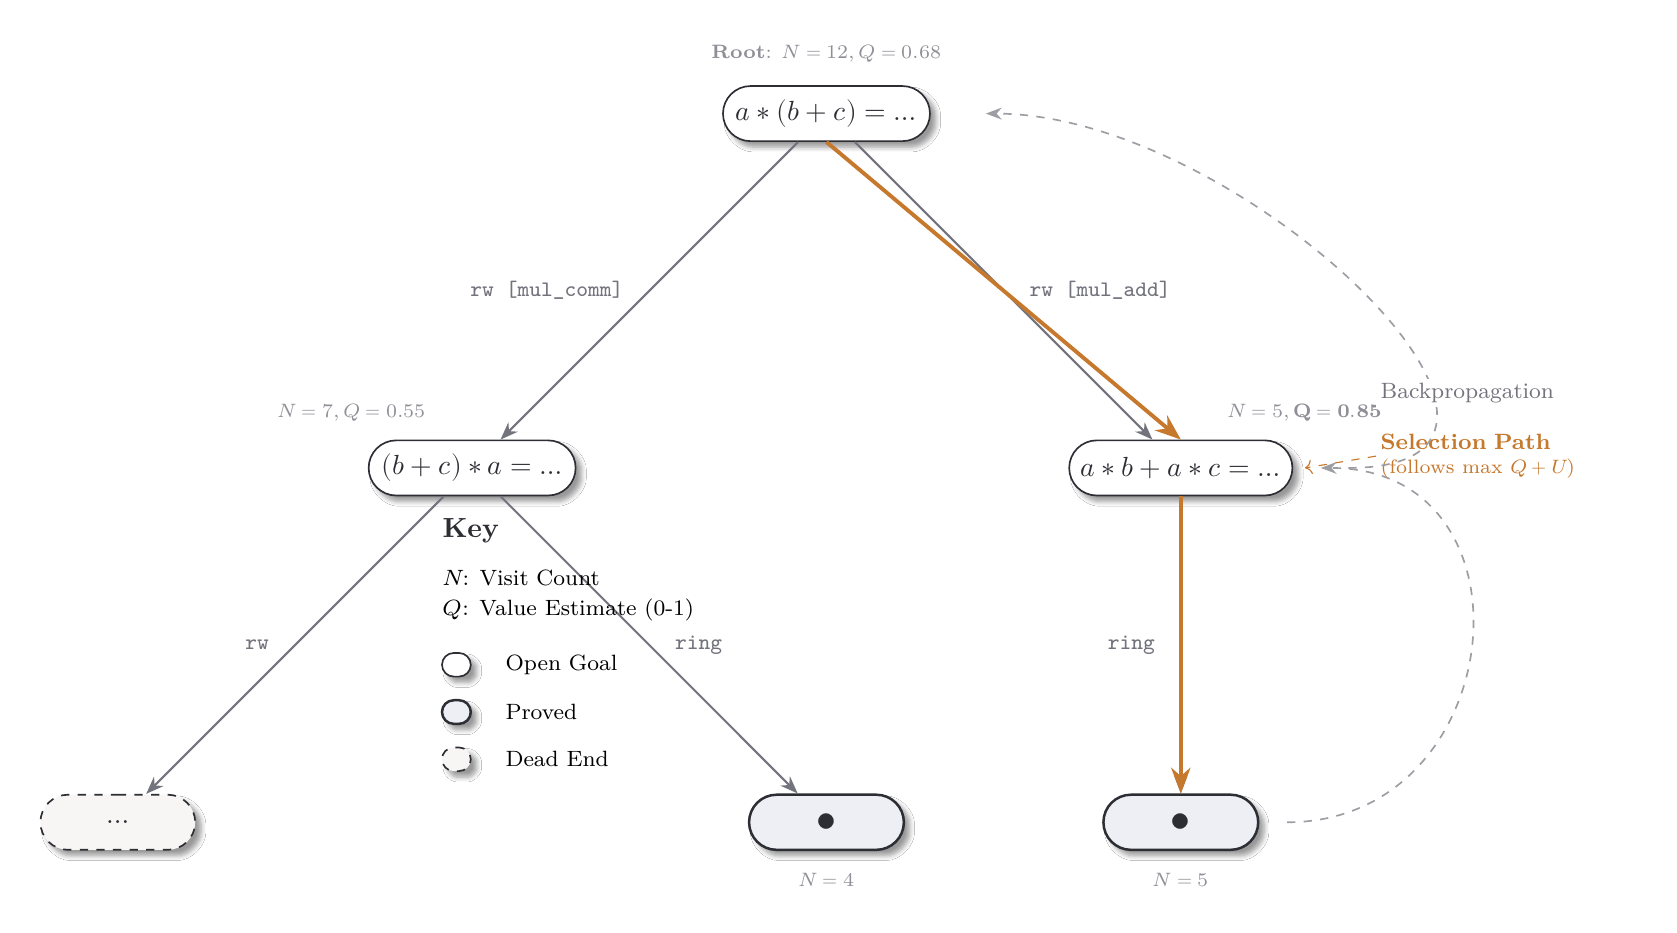
\begin{tikzpicture}[
    level distance=4.5cm,
    sibling distance=9.0cm,
    every node/.style={font=\normalfont},
    edge from parent/.style={tactic},
    label distance=6pt,
    show background rectangle,
    background rectangle/.style={fill=white}
]

\tikzset{visit/.style={annot, font=\normalfont\scriptsize, inner sep=2pt, fill=white, fill opacity=0.8, rounded corners=2pt}}

% Main MCTS Tree
\node[goal, label={[visit]above:{\textbf{Root}: $N=12, Q=0.68$}}] (root) {$a*(b+c)=\ldots$}
    child {
        node[goal, label={[visit]above left:{$N=7, Q=0.55$}}] (n1) {$(b+c)*a=\ldots$}
        child {
            node[dead] (n1a) {$\ldots$}
            edge from parent node[left, tacticlabel, xshift=-0.2cm] {rw}
        }
        child {
            node[terminal, label={[visit]below:{$N=4$}}] (n1b) {\Large$\bullet$}
            edge from parent node[right, tacticlabel, xshift=0.2cm] {ring}
        }
        edge from parent node[left, tacticlabel, xshift=-0.2cm] {rw [mul\_comm]}
    }
    child {
        node[goal, label={[visit]above right:{$N=5, \mathbf{Q=0.85}$}}] (n2) {$a*b+a*c=\ldots$}
        child {
            node[terminal, label={[visit]below:{$N=5$}}] (n2a) {\Large$\bullet$}
            edge from parent node[left, tacticlabel, xshift=-0.2cm] {ring}
        }
        edge from parent node[right, tacticlabel, xshift=0.2cm] {rw [mul\_add]}
    };

% Selection path highlight (Orange Arrow)
\draw[selected] (root.south) -- (n2.north);
\draw[selected] (n2.south) -- (n2a.north);

% Explicit label for the selection path
\node[
    annotbg,
    text=highlight,
    anchor=west,
    text width=3.2cm,
    align=left
] (sel_label) at ([xshift=1.05cm, yshift=0.15cm]n2.east) {\textbf{Selection Path}\\[-1pt]\scriptsize (follows max $Q + U$)};
\draw[->, highlight, dashed] (sel_label.west) -- ([xshift=0.15cm]n2.east);

% Backpropagation arrows (Curved for elegance)
\draw[backprop] ([xshift=0.35cm]n2a.east) to[out=0, in=0, looseness=1.6] ([xshift=0.35cm]n2.east);
\draw[backprop] ([xshift=0.70cm]n2.east) to[out=0, in=0, looseness=1.3] ([xshift=0.70cm]root.east);
\node[annotbg, anchor=west, text=muted] at ([xshift=1.05cm, yshift=0.95cm]n2.east) {Backpropagation};

% Legend / Key
\begin{scope}[shift={(-5.0, -6.5)}]
    \node[paneltitle, anchor=west] at (0, 1.2) {Key};
    
    % N and Q explanation
    \node[right, font=\footnotesize] at (0, 0.6) {$N$: Visit Count};
    \node[right, font=\footnotesize] at (0, 0.2) {$Q$: Value Estimate (0-1)};
    
    % Node types
    \node[goal, minimum width=0.6cm, minimum height=0.3cm] (lg) at (0.3, -0.5) {};
    \node[right, font=\footnotesize] at (0.8, -0.5) {Open Goal};

    \node[terminal, minimum width=0.6cm, minimum height=0.3cm] (lt) at (0.3, -1.1) {};
    \node[right, font=\footnotesize] at (0.8, -1.1) {Proved};
    
    \node[dead, minimum width=0.6cm, minimum height=0.3cm] (ld) at (0.3, -1.7) {};
    \node[right, font=\footnotesize] at (0.8, -1.7) {Dead End};
\end{scope}

\end{tikzpicture}
\end{document}
